\chapter{Semi-supervised Verfahren}
\label{chap:ssdml}

\section{Semi-supervised Learning}
\label{sec:ssl}

Das supervised Learning verwendet gelabelte Daten zum Training eines Modells, während das unsupervised Learning ohne vorgegebene Labels auskommt. Das \acl{SSL} hingegen verfolgt eine supervised Aufgabe wie die Klassifikation, nutzt dafür jedoch zusätzlich ungelabelte Daten \cite{van_engelen_survey_2019}. In der Notation dieser Arbeit umfasst der Trainingspool $\mathcal{X}=\{\bm{x}_i\}_{i=1}^{N}$ gelabelte Bilder mit Index in $\mathcal{I}_{\mathrm{L}}$, deren Klassenlabel $y_i\in\{1,\dots,C\}$ bekannt ist. Für die übrigen Bilder mit Index in $\mathcal{I}_{\mathrm{U}}=\{1,\dots,N\}\setminus\mathcal{I}_{\mathrm{L}}$ ist $y_i$ unbekannt. Im Trainingspool kommen $C$ Klassen vor. Die gelabelten Klassen bilden die Menge $\mathcal{C}_{\mathrm{L}}=\{y_i:i\in\mathcal{I}_{\mathrm{L}}\}$. Klassen, die ausschließlich ungelabelt vorkommen, fehlen in $\mathcal{C}_{\mathrm{L}}$, sodass $|\mathcal{C}_{\mathrm{L}}|=C$ nur gilt, wenn jede Klasse gelabelte Bilder hat. Ob ungelabelte Daten helfen, hängt davon ab, wie die Merkmalsverteilung $p(\bm{x})$ mit der bedingten Klassenverteilung $p(y\mid\bm{x})$ zusammenhängt \cite{van_engelen_survey_2019}.

Die Nutzung ungelabelter Daten im \ac{SSL} beruht auf Annahmen über die Struktur und Verteilung der Daten. Die \emph{Smoothness-Annahme} besagt, dass nahe beieinanderliegende Punkte im Eingaberaum dasselbe Label haben sollten. Nach der \emph{Mannigfaltigkeitsannahme} gehören Punkte auf derselben niedrigdimensionalen Mannigfaltigkeit zur gleichen Klasse. Die \emph{Low-Density-Annahme} besagt dagegen, dass Entscheidungsgrenzen durch Bereiche geringer Datendichte verlaufen sollten \cite{van_engelen_survey_2019}. Die Übersicht beschreibt diese drei Annahmen als spezielle Formen der \emph{Cluster-Annahme}, nach der Punkte desselben Clusters zur gleichen Klasse gehören \cite{van_engelen_survey_2019}. Abbildung \ref{fig:ssl:annahmen} veranschaulicht, welche ungelabelten Punkte unter den jeweiligen Annahmen derselben Klasse zugeordnet werden.

\begin{figure}[tbp]
  \centering
  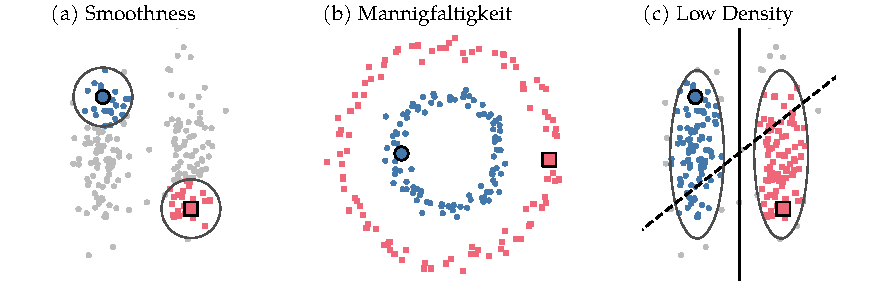
\includegraphics{neu/ssl_annahmen}
  \caption[Annahmen des \acs{SSL} an synthetischen Daten]{Annahmen des \acs{SSL} an synthetischen Daten nach \cite{van_engelen_survey_2019}. Groß und schwarz umrandet: gelabelte Punkte. Farbig: ungelabelte Punkte, die nach der Annahme dem gelabelten Punkt derselben Farbe ähneln, grau: übrige. (a) Kreise: Umgebungen der gelabelten Punkte. (c) Ellipsen: Bereiche hoher Dichte bis zu zwei Standardabweichungen um die Klassenmitten, durchgezogen: eine Entscheidungsgrenze im Bereich geringer Dichte, gestrichelt: Mittelsenkrechte der gelabelten Punkte als Grenze ohne ungelabelte Punkte.}
  \label{fig:ssl:annahmen}
\end{figure}

In dieser Arbeit gelten die Annahmen nicht im Eingaberaum der Rohbilder, sondern in dem Raum, in dem die Ähnlichkeit gemessen wird. Ein ungelabeltes Foto eines Automodells kann nur dann über seine Nachbarn einer Klasse zugeordnet werden, wenn diese Nachbarn im Merkmals- oder Embedding-Raum überwiegend dasselbe Automodell zeigen. Ob das zutrifft, hängt von der Datenverteilung und von der Repräsentation ab. Zu Beginn des Trainings ist daher entscheidend, wie gut das vortrainierte Modell die Trainingsklassen bereits trennt. Die Annahmen müssen deshalb im konkreten Fall geprüft werden. Im \ac{DML} kommt eine weitere Annahme hinzu. Was ein Modell an den ungelabelten Bildern lernt, bei Autos etwa eine geringere Empfindlichkeit gegenüber dem Blickwinkel, der Lackfarbe und dem Hintergrund, muss sich auf ungesehene Klassen übertragen.

Ein \emph{induktives} Verfahren lässt sich anders als ein \emph{transduktives} ohne weiteres Training auf neue Daten anwenden \cite{van_engelen_survey_2019}. Für diese Arbeit ist entscheidend, dass \ac{DML} ein induktives Modell verlangt, denn getestet wird auf Bildern oder sogar Klassen, die im Training nicht vorkamen. Ein transduktiver Baustein kann aber Teil eines induktiven Verfahrens sein. Bei der Übertragung auf tiefe Netze dient \ac{LP} als transduktiver Zwischenschritt, der den ungelabelten Beispielen Pseudo-Labels zuweist. Mit diesen wird anschließend ein induktives Modell trainiert \cite{iscen_label_2019}.

Induktive Verfahren werden danach unterschieden, wie die ungelabelten Daten in sie eingehen. Bei der \emph{unsupervised Vorverarbeitung} werden sie in einem eigenen Schritt vor dem supervised Training genutzt, beispielsweise zum Vortraining neuronaler Netze. \emph{Wrapper-Verfahren} weisen den ungelabelten Daten dagegen Pseudo-Labels zu, um sie anschließend für das supervised Training zu nutzen. \emph{Intrinsisch semi-supervised Verfahren} erweitern das Lernverfahren selbst, etwa um einen zusätzlichen Term im Trainingsziel \cite{van_engelen_survey_2019}. Bei neuronalen Netzen lassen sich ungelabelte Daten so über einen gewichteten Regularisierungsterm einbeziehen, der zur supervised Verlustfunktion hinzukommt \cite{weston_deep_2012, hoffer_semi-supervised_2018}. In der Notation dieser Arbeit lautet ein solches Trainingsziel \cite{weston_deep_2012, hoffer_semi-supervised_2018}
\begin{equation}
  \mathcal{L}=\mathcal{L}_{\mathrm{sup}}+w_{\mathrm{reg}}\,\mathcal{L}_{\mathrm{reg}}.
  \label{eq:ssl:ziel}
\end{equation}
Dabei ist $\mathcal{L}_{\mathrm{sup}}$ eine \ac{DML}-Verlustfunktion aus Abschnitt \ref{sec:verluste} auf den gelabelten Bildern. Der \ac{SSL}-Term $\mathcal{L}_{\mathrm{reg}}$ bezieht die ungelabelten Bilder ein und $w_{\mathrm{reg}}\ge0$ ist sein Gewicht. DINOv2 wurde mit Self-supervised Learning auf externen Daten vortrainiert, was einer unsupervised Vorverarbeitung entspricht \cite{oquab_dinov2_2023}. In dieser Arbeit liefert dieses Vortraining die festen Merkmale für alle Experimente.

Zu den drei Gruppen gehören weitere Verfahren, etwa das Co-Training, störungsbasierte Ansätze wie Mean Teacher, generative Modelle und Semi-supervised Support Vector Machines \cite{van_engelen_survey_2019}. 

\section{Evaluation von semi-supervised Verfahren}
\label{sec:ssl:evaluation}

Wie groß der Vorteil von \ac{SSL} in der Bildklassifikation unter vergleichbaren Versuchsbedingungen ausfällt, wurde mit mehreren \ac{SSL}-Verfahren bei derselben Netzarchitektur und einem einheitlichen Trainingsablauf in einer Vergleichsarbeit untersucht. Sowohl die supervised Baseline als auch jedes \ac{SSL}-Verfahren wurden mit jeweils 1000 Versuchen zur Hyperparameteroptimierung abgestimmt. Unter diesen Bedingungen reduzierte zum Beispiel das $\Pi$-Model den Testfehler auf CIFAR-10 mit 4000 Labels von \qty{20.26}{\percent} auf \qty{16.37}{\percent}. Dieselbe Studie stellt dem einen früher berichteten Rückgang von \qty{34.85}{\percent} auf \qty{12.36}{\percent} gegenüber, der von einer deutlich schwächeren supervised Baseline ausging. Ein Netz, das zunächst auf ImageNet vortrainiert und anschließend mit 4000 gelabelten CIFAR-10-Bildern angepasst wurde, erreichte einen geringeren Testfehler als alle untersuchten \ac{SSL}-Verfahren derselben Architektur \cite{oliver_realistic_2018}.

Auch die Validierungsmenge entscheidet darüber, wie aussagekräftig ein Vergleich ist. Auf SVHN standen in vielen Arbeiten nur 1000 gelabelten Trainingsbildern rund 7000 gelabelte Validierungsbilder gegenüber, ein Verhältnis, das in der Praxis kaum vorkommt. Bei 100 Validierungsbildern schwankten die geschätzten Fehlerraten dagegen so stark, dass sich die Verfahren kaum noch zuverlässig vergleichen ließen. Außerdem kann \ac{SSL} schlechter abschneiden als die supervised Baseline, wenn die ungelabelten Daten Klassen ohne gelabelte Beispiele enthalten. Das zeigte ein Versuch mit den sechs Tierklassen von CIFAR-10 als gelabelter Aufgabe und zusätzlich mit ungelabelten Daten aus vier Klassen, von denen schrittweise weniger zu den gelabelten gehörten. Im Extremfall stammten sie nur aus den vier Fahrzeugklassen. Die Hyperparameter wurden für diesen Versuch allerdings nicht neu gesucht \cite{oliver_realistic_2018}.

In diesen Versuchen näherten sich die Verfahren mit wachsender Zahl der Labels einander an, wobei sie mit wenigen Labels am weitesten auseinander lagen. Über Datensätze mit unterschiedlich vielen Klassen hinweg lässt sich das Label-Budget als Zahl gelabelter Bilder je Klasse vergleichen. Die 4000 Labels, mit denen Verfahren auf CIFAR-10 häufig getestet wurden, entsprechen 400 Bildern je Klasse \cite{oliver_realistic_2018}. Im \ac{SSDML} wurden für Cars196 und \ac{CUB} dagegen jeweils nur fünf Bilder je Klasse verwendet \cite{dutta_semi-supervised_2021, zhuang_deep_2021}.

Die Frage nach Klassen, die nur im ungelabelten Pool vorkommen, ist inzwischen differenzierter beantwortet. In vielen früheren Versuchen blieb die Zahl der ungelabelten Bilder fest, sodass ein größerer Anteil unbekannter Klassen zugleich weniger ungelabelte Bilder bekannter Klassen bedeutete. Ohne diese Kopplung sank die Genauigkeit der meisten Verfahren mit wachsendem Anteil unbekannter Klassen weiterhin, aber unterschiedlich stark \cite{he_reevaluating_2025}. Auf den fine-grained Datensätzen Semi-Aves und Semi-Fungi kamen Bilder weiterer Arten zu den ungelabelten Bildern bekannter Arten hinzu. Ohne Vortraining halfen zusätzliche ungelabelte Daten aus unbekannten Klassen bei einigen Verfahren. Bei vortrainierten Modellen verschlechterten sie dagegen häufig die Ergebnisse \cite{su_realistic_2021}. Für Hypothese H3 aus Kapitel \ref{chap:einleitung} folgt daraus zweierlei. Ein Befund zu H3 hängt davon ab, ob Bilder fremder Klassen ungelabelte Bilder bekannter Klassen ersetzen oder zu ihnen hinzukommen. Außerdem ist ein Schaden nach diesen Befunden bei einem vortrainierten Modell wie DINOv2 eher zu erwarten als ohne Vortraining. 

Mit stark vortrainierten \ac{ViT}-Modellen stellt sich die Frage nach dem Nutzen ungelabelter Daten neu. Auf Benchmarks wie CIFAR-10 genügt bereits ein linearer Klassifikator auf eingefrorenen Merkmalen, um mit wenigen Labels eine hohe Genauigkeit zu erreichen. Klassische \ac{SSL}-Verfahren erzielten gegenüber rein supervised Fine-Tuning-Verfahren jedoch auch auf schwierigeren Aufgaben oft nur geringe Leistungsgewinne. Auf anspruchsvolleren Aufgaben liefert parametereffizientes Fine-Tuning allein mit gelabelten Daten häufig bessere Ergebnisse als die untersuchten \ac{SSL}-Verfahren. Durch die Kombination der Pseudo-Labels verschiedener solcher Modelle lassen sich dort jedoch zusätzliche Gewinne mit ungelabelten Daten erzielen \cite{zhang_revisiting_2025}. Ob diese Befunde für das \ac{DML} mit ungesehenen Testklassen gelten, ist offen.

\section{Entropieminimierung, Pseudo-Labels und Self-Training}
\label{sec:selftraining}

\subsection{Entropieminimierung und Pseudo-Labels}
\label{sec:entropie}

Ausgangspunkt der Entropieminimierung ist, dass ein ungelabelter Punkt in der bedingten Log-Likelihood wegen $\sum_{c\in\mathcal{C}_{\mathrm{L}}}p_{ic}=1$ mit $p_{ic}=p(c\mid\bm{x}_i;\bm{\theta})$ nur den Summanden $\log 1=0$ beiträgt \cite{grandvalet_semi-supervised_2005}. Das Verfahren ergänzt die negative bedingte Log-Likelihood der gelabelten Punkte, die dort die Rolle von $\mathcal{L}_{\mathrm{sup}}$ in Gleichung \eqref{eq:ssl:ziel} übernimmt, um einen \ac{SSL}-Term, in der Notation dieser Arbeit \cite{grandvalet_semi-supervised_2005}
\begin{equation}
  \mathcal{L}_{\mathrm{reg}}^{\mathrm{Ent}}=-\sum_{i\in\mathcal{I}_{\mathrm{U}}}\sum_{c\in\mathcal{C}_{\mathrm{L}}}p_{ic}\log p_{ic}.
  \label{eq:entmin}
\end{equation}
Der Term minimiert die Entropie der Klassenvorhersagen für ungelabelte Datenpunkte und begünstigt damit eine hohe Konfidenz bei der Zuordnung zu einer Klasse. Bei einem ausreichend regularisierten Modell kann die Konfidenz nahe der Entscheidungsgrenze nicht beliebig hoch sein. Die Entropieminimierung begünstigt daher Entscheidungsgrenzen in Bereichen geringer Datendichte und folgt damit der Low-Density-Annahme \cite{grandvalet_semi-supervised_2005}.

Pseudo-Labeling kommt ohne eigenen Entropieterm aus. Für die ungelabelten Bilder eines Batches wird bei jeder Gewichtsaktualisierung die jeweils wahrscheinlichste Klasse zum One-hot-Ziel. Der supervised Verlust behandelt dieses Pseudo-Label wie ein echtes Label. Der Verlustterm der ungelabelten Bilder erhält aber ein eigenes Gewicht, das zunächst null ist und dann linear auf einen Endwert steigt. Gedeutet wird dieses Vorgehen dort als eine Form der Entropieminimierung \cite{lee_pseudo-label_2013}.

\subsection{Self-Training und Teacher-Student}
\label{sec:teacher-student}

Beim \emph{Self-Training} erweitert ein Modell seine gelabelte Trainingsmenge aus den eigenen Vorhersagen, denn nach jeder Runde gelten ausgewählte Vorhersagen für ungelabelte Daten, etwa die mit der höchsten Konfidenz, als Pseudo-Labels der nächsten Runde \cite{yarowsky_unsupervised_1995, van_engelen_survey_2019}. Das Risiko solcher Verfahren, der \emph{Confirmation Bias}, liegt darin, dass sich falsche Pseudo-Labels festsetzen, weil das Modell aus seinen eigenen Fehlern lernt. Mixup und genügend gelabelte Bilder in jedem Batch brachten Pseudo-Labeling in den dortigen Versuchen zur Bildklassifikation auf das Niveau der Konsistenzregularisierung oder darüber \cite{arazo_2020}.

Bei Noisy Student erzeugt in jeder Runde das zuletzt trainierte Modell als Teacher die Pseudo-Labels, aus denen ein neuer Student lernt. Rauschen in Form von Augmentierung, Dropout und stochastischer Tiefe wirkt dabei beim Training beider Modelle, nicht aber beim Erzeugen der Pseudo-Labels \cite{xie_self-training_2019}. Mean Teacher gehört zur Konsistenzregularisierung, bei der ein Modell für verschiedene Störungen desselben Bildes dieselbe Vorhersage liefern soll. Dessen Teacher ist kein getrennt trainiertes Modell, sondern ein \ac{EMA} der Student-Gewichte, $\bm{\theta}'\leftarrow\beta\,\bm{\theta}'+(1-\beta)\,\bm{\theta}$ mit $\beta$ nahe eins. Der Student wird so trainiert, dass seine Vorhersage möglichst wenig von der des Teachers abweicht \cite{tarvainen_weight-averaged_2017}. FixMatch verbindet Pseudo-Labels und Konsistenzregularisierung über zwei unterschiedlich stark augmentierte Ansichten desselben ungelabelten Bildes und eine Konfidenzschwelle \cite{sohn_fixmatch_2020}.

Mean Teacher und FixMatch verlangen mit ihrem Konsistenzterm keine gleichen Labels für nahe Bilder, sondern gleiche Vorhersagen für veränderte Fassungen desselben Bildes \cite{tarvainen_weight-averaged_2017, sohn_fixmatch_2020}. Das entspricht der bei Bildern üblichen, abgeschwächten Form der Smoothness-Annahme \cite{van_engelen_survey_2019}. 

\section{Graphbasierte Verfahren}
\label{sec:graph}

\subsection{Graphen und Laplace-Matrix}

Die folgende Darstellung der Graphkonstruktion orientiert sich an der Übersicht in \textcite{van_engelen_survey_2019}. Graphbasierte Verfahren repräsentieren gelabelte und ungelabelte Punkte als Knoten eines Graphen, dessen Kanten Ähnlichkeiten beschreiben. Die Gewichtsmatrix $\bm{W}\in\mathbb{R}^{N\times N}$ enthält für jede Kante ein nichtnegatives Gewicht $W_{ij}$ und für alle übrigen Paare null. Verbreitet sind \ac{kNN}-Graphen, in denen jeder Punkt mit seinen $k_{\mathrm{NN}}$ nächsten Nachbarn verbunden ist. Weil diese Beziehung nicht symmetrisch ist, wird für eine Kante entweder verlangt, dass einer der beiden Punkte zu den Nachbarn des anderen zählt, oder dass beide wechselseitig Nachbarn sind \cite{van_engelen_survey_2019}. Die Gewichte sind beispielsweise binär \cite{hoi_semi-supervised_2010} oder ergeben sich über einen Kern aus der Distanz, etwa $W_{ij}=\exp(-\gamma\lVert\bm{x}_i-\bm{x}_j\rVert_2^2)$ \cite{van_engelen_survey_2019}. Im Folgenden sind die Graphen ungerichtet, also $\bm{W}=\bm{W}^{\top}$, ohne Selbstkanten ($W_{ii}=0$). Die Gradmatrix $\bm{D}$ ist diagonal mit den Knotengraden $D_{ii}=\sum_j W_{ij}$ und die Graph-Laplace-Matrix ist $\bm{L}=\bm{D}-\bm{W}$. Summiert über die Spalten einer Matrix $\bm{F}\in\mathbb{R}^{N\times|\mathcal{C}_{\mathrm{L}}|}$ ergibt die quadratische Form von $\bm{L}$ den \emph{Laplace-Term} \cite{hoi_semi-supervised_2010, belkin_manifold_2006}
\begin{equation}
  \operatorname{tr}(\bm{F}^{\top}\bm{L}\bm{F})=\tfrac{1}{2}\sum_{i,j}W_{ij}\,\lVert\bm{F}_{i:}-\bm{F}_{j:}\rVert_2^2 .
  \label{eq:laplace}
\end{equation}
Der Term ist klein, wenn verbundene Knoten ähnliche Zeilen in $\bm{F}$ haben. Damit begünstigt er ähnliche Vorhersagen für benachbarte Punkte und folgt der Smoothness-Annahme. Da der Graph auch weiter entfernte Punkte über mehrere Kanten verbinden kann, lässt sich die Glättung entlang der durch den Graphen angenäherten Mannigfaltigkeitsstruktur fortsetzen \cite{zhou_learning_2003, belkin_manifold_2006, van_engelen_survey_2019}. Auf den Knoten mit positivem Grad vergleicht die symmetrisch normierte Variante $\bm{L}_{\mathrm{sym}}=\bm{I}-\bm{D}^{-1/2}\bm{W}\bm{D}^{-1/2}$ die mit $1/\sqrt{D_{ii}}$ skalierten Zeilen von $\bm{F}$ \cite{zhou_learning_2003, belkin_manifold_2006}. Ohne die Normierung können Knoten mit vielen oder starken Kanten einen größeren Einfluss auf den Laplace-Term haben. Die Skalierung mit $1/\sqrt{D_{ii}}$ dämpft diesen Einfluss \cite{van_engelen_survey_2019}. Für diese Arbeit ist entscheidend, wie viele Kanten eines Graphen innerhalb einer Klasse verlaufen. Verbindet er Bilder ähnlicher, aber verschiedener Klassen, verlangt der Laplace-Term ähnliche Werte genau dort, wo die Labels wechseln.

\subsection{Label Propagation}
\label{sec:lp}

Label Propagation überträgt Labelinformationen entlang der Kanten auf ungelabelte Knoten. Jeder Knoten erhält wiederholt die mit den Kantengewichten gewichteten Label-Scores seiner Nachbarn, die Scores werden normiert und die gelabelten Knoten werden nach jedem Schritt auf ihr bekanntes Label zurückgesetzt \cite{zhu_learning_2002}. Bei der Variante mit lokaler und globaler Konsistenz bleiben die Label-Scores der gelabelten Knoten veränderlich. Ein quadratischer Strafterm bestraft Abweichungen von den Ausgangslabels \cite{zhou_learning_2003}. Dadurch kann das Verfahren weniger empfindlich auf fehlerhafte Labels reagieren als die klassische Label Propagation mit festgehaltenen Labels. Diese Variante wird auch als Label Spreading bezeichnet \cite{van_engelen_survey_2019,pedregosa_scikit-learn_2011}. Die Matrix $\bm{Y}\in\mathbb{R}^{N\times|\mathcal{C}_{\mathrm{L}}|}$ enthält die One-hot-Labels der gelabelten Knoten. Jede Spalte entspricht einer Klasse $c\in\mathcal{C}_{\mathrm{L}}$. Die Zeilen der ungelabelten Knoten enthalten nur Nullen. Mit $\bm{S}=\bm{D}^{-1/2}\bm{W}\bm{D}^{-1/2}$ und $0<\alpha<1$ wird dort \cite{zhou_learning_2003}
\begin{equation}
  \bm{F}^{(t+1)}=\alpha\bm{S}\bm{F}^{(t)}+(1-\alpha)\bm{Y}
  \quad\xrightarrow{t\to\infty}\quad
  \bm{F}^{*}=(1-\alpha)(\bm{I}-\alpha\bm{S})^{-1}\bm{Y}
  \label{eq:lp}
\end{equation}  
iteriert. Je näher $\alpha$ an eins liegt, desto stärker hängen die Label-Scores von den Nachbarn ab und desto schwächer hängen sie von den Ausgangslabels ab, die in jedem Schritt mit dem Gewicht $1-\alpha$ eingehen. Das Pseudo-Label eines ungelabelten Knotens entspricht der Klasse mit dem größten Wert in seiner Zeile von $\bm{F}^{*}$. Der Fixpunkt minimiert eine Zielfunktion aus dem Laplace-Term mit $\bm{L}_{\mathrm{sym}}$ und der quadratischen Abweichung von $\bm{Y}$ \cite{zhou_learning_2003}.

Verlaufen zwischen den Klassen wenige Kanten, können Labels entlang einer Mannigfaltigkeit auch Punkte derselben Klasse erreichen, die weit von jedem gelabelten Punkt entfernt sind. Wo zwei Klassen ineinander übergehen, gelangen Labels leicht über die verbindenden Kanten in die falsche Klasse. Nur auf der Indexmenge $\mathcal{I}_{+}=\{i:\sum_{c\in\mathcal{C}_{\mathrm{L}}}F^{*}_{ic}>0\}$ entsteht durch $p_{ic}=F^{*}_{ic}/\sum_{c'\in\mathcal{C}_{\mathrm{L}}}F^{*}_{ic'}$ eine Verteilung \cite{iscen_label_2019}. Mit $0\log0=0$ lautet die Konfidenz für $|\mathcal{C}_{\mathrm{L}}|>1$ in der Notation dieser Arbeit \cite{iscen_label_2019}
\begin{equation}
  \omega_i=1-\frac{H(\bm{p}_i)}{\log|\mathcal{C}_{\mathrm{L}}|},\qquad H(\bm{p}_i)=-\sum_{c\in\mathcal{C}_{\mathrm{L}}}p_{ic}\log p_{ic}.
  \label{eq:lp-weight}
\end{equation}
Sie ist bei einer Gleichverteilung null und bei einer eindeutigen Zuordnung eins. Eine Verteilung auf mehrere Klassen senkt sie, bei vielen bekannten Klassen kann aber schon eine Verteilung auf nur zwei Klassen einen hohen Wert ergeben. Ein hoher Wert von $\omega_i$ ist deshalb kein Nachweis eines richtigen Pseudo-Labels. Auch falsche Pseudo-Labels erreichten in der ursprünglichen Arbeit hohe Werte. Die Konfidenz wird dort zusätzlich so zu $\tilde\omega_i$ skaliert, dass ihr Maximum über alle Bilder eins ist. Diese vorherige Arbeit, die \acl{LP} auf tiefe Netze überträgt, bezeichnet die Propagation als Diffusion und lässt sie mit dem Training abwechseln \cite{iscen_label_2019}. Nach einem supervised Warm-up werden dort alle Trainingsbilder eingebettet und aus den Embeddings entsteht ein dünner Graph, in der Notation dieser Arbeit mit \cite{iscen_label_2019}
\begin{equation}
  \hat{W}_{ij}=[s_{ij}]_+^{\xi}\ \text{für } j\in\mathcal{V}_{k_{\mathrm{NN}}}(i),\qquad \bm{W}=\hat{\bm{W}}+\hat{\bm{W}}^{\top}.
  \label{eq:lp-graph}
\end{equation}
Dabei ist $\mathcal{V}_{k_{\mathrm{NN}}}(i)$ die Menge der $k_{\mathrm{NN}}$ nächsten Nachbarn von $i$ ohne $i$ selbst. Alle übrigen Einträge von $\hat{\bm{W}}$ sind null. Der Parameter $\xi$ ist ein Exponent, der hohe Ähnlichkeiten betont. Das Verfahren der konjugierten Gradienten löst dort das lineare System $(\bm{I}-\alpha\bm{S})\bm{F}=\bm{Y}$, ohne die dicht besetzte Inverse aus Gleichung \eqref{eq:lp} zu bilden, die bei großen Graphen nicht praktikabel ist. Aus der zeilennormierten Lösung ergeben sich das Pseudo-Label $\hat{y}_i=\argmax_{c\in\mathcal{C}_{\mathrm{L}}}p_{ic}$ und die Konfidenz $\omega_i$ \cite{iscen_label_2019}. Der Faktor $1-\alpha$ aus Gleichung \eqref{eq:lp} wird bei der Klassifikation weggelassen \cite{zhou_learning_2003,iscen_label_2019}. Die ursprüngliche Arbeit zur Anwendung von \ac{LP} auf tiefe Netze trainiert das Netz anschließend mit einer gewichteten Kreuzentropie auf gelabelten und pseudo-gelabelten Bildern. Die Gewichte gleichen unterschiedlich große Klassen aus und dämpfen zusätzlich unsichere Pseudo-Labels über die Konfidenz $\omega_i$. Der Graph und die Pseudo-Labels werden nach jeder Epoche aus den aktualisierten Embeddings neu berechnet und die vorherige Arbeit verwendet $k_{\mathrm{NN}}=50$, $\xi=3$ und $\alpha=\num{0.99}$ \cite{iscen_label_2019}.

\subsection{Graph-Regularisierung tiefer Netze}
\label{sec:weston}

Statt Labels über einen Graphen zu verteilen, kann der Laplace-Term aus Gleichung \eqref{eq:laplace} auch direkt als Regularisierer dienen. Die Mannigfaltigkeitsregularisierung ergänzt eine Zielfunktion um einen gewichteten Term $\operatorname{tr}(\bm{F}^{\top}\bm{L}\bm{F})$. Dabei enthält $\bm{F}$ die Vorhersagen für alle gelabelten und ungelabelten Datenpunkte. Der Term bestraft unterschiedliche Vorhersagen auf stark verbundenen Graphknoten. Dadurch wird eine Vorhersagefunktion begünstigt, die entlang der durch den Graphen approximierten Geometrie der Daten glatt verläuft \cite{belkin_manifold_2006}.

Die Embedding-Regularisierung überträgt diese Idee auf tiefe Netze. Sie addiert zum supervised Verlust eine Variante des Contrastive Loss aus Abschnitt \ref{sec:verluste:paare}, deren anziehender Teil auf im Graphen verbundene Paare und deren abstoßender Teil auf Paare ohne Kante wirkt. Ohne den abstoßenden Teil wäre dieser Verlust auf den ungelabelten Paaren schon mit $d_{ij}=0$ für alle Paare minimal. Abwechselnd erhalten ein gelabeltes Beispiel einen Schritt auf dem supervised Verlust, ein benachbartes Paar aus dem Graphen einen Schritt auf dem anziehenden Teil und ein Paar mit einem zufällig gezogenen ungelabelten Beispiel einen Schritt auf dem abstoßenden Teil \cite{weston_deep_2012}.

\section{Semi-supervised Metric Learning}
\label{sec:ssml}

\subsection{Graph-Regularisierung einer Metrik}
\label{sec:lrml}

\ac{LRML} verwendet den Laplace-Term als Regularisierer für eine Mahalanobis-Metrik. Aus allen gelabelten und ungelabelten Punkten wird dort mit der euklidischen Distanz ein ungewichteter \ac{kNN}-Graph gebaut, in dem $W_{ij}=1$ gilt, wenn $i$ unter den $k_{\mathrm{NN}}$ nächsten Nachbarn von $j$ ist oder umgekehrt. Die Metrik soll benachbarte Punkte auch nach der Transformation nahe beieinander halten. In der Notation dieser Arbeit lautet der Regularisierer \cite{bellet_survey_2014, hoi_semi-supervised_2010}
\begin{equation}
  \mathcal{L}_{\mathrm{reg}}^{\mathrm{LRML}}(\bm{M})=\tfrac{1}{2}\sum_{i,j}W_{ij}\,d_{\bm{M}}^{2}(\bm{x}_i,\bm{x}_j)=\operatorname{tr}(\bm{X}\bm{L}\bm{X}^{\top}\bm{M}).
  \label{eq:lrml}
\end{equation}
Dabei ist $\bm{X}=[\bm{x}_1,\dots,\bm{x}_N]$ die Matrix mit den Datenpunkten als Spalten. Die Gleichung gilt für $\bm{L}=\bm{D}-\bm{W}$. Für die Anwendung ist dort auch $\bm{L}_{\mathrm{sym}}$ vorgesehen, mit der die Retrieval-Experimente bei $k_{\mathrm{NN}}=6$ rechnen \cite{hoi_semi-supervised_2010}. Der Regularisierer wird mit zwei Termen für gelabelte Paare kombiniert, die die Abstände ähnlicher Paare verkleinern und die Abstände unähnlicher Paare vergrößern. Der Laplace-Term selbst verwendet keine Labels, sondern begünstigt kleine Abstände zwischen Graphnachbarn. Damit orientiert sich \ac{LRML} an der Smoothness-Annahme und berücksichtigt über den Nachbarschaftsgraphen die lokale Datenstruktur im Sinne der Mannigfaltigkeitsannahme aus Abschnitt \ref{sec:ssl} \cite{bellet_survey_2014, hoi_semi-supervised_2010}.

Neben \ac{LRML} wurden weitere Verfahren entwickelt, die die Struktur ungelabelter Daten beim Metric Learning berücksichtigen. Diese unterscheiden sich unter anderem in der Konstruktion des Nachbarschaftsgraphen und in der Wahl des Mannigfaltigkeitsregularisierers \cite{bellet_survey_2014}. Einer der Ansätze bestimmt beispielsweise zunächst, wie sich jeder Datenpunkt
im ursprünglichen Merkmalsraum aus seinen nächsten Nachbarn
rekonstruieren lässt. Ein Regularisierungsterm bestraft
anschließend Abweichungen von diesen Rekonstruktionsbeziehungen
im transformierten Raum \cite{baghshah_semi-supervised_2009}.

Es gibt noch weitere Verfahren, von denen hier einige aufgezählt werden. Das Verfahren \ac{RSSML} erweitert die Laplace-Regularisierung um Gauß-Ähnlichkeiten zwischen benachbarten Punkten und Dichtegewichte. Der Regularisierer wird mit einem Triplet-Hinge-Verlust kombiniert \cite{wang_semi-supervised_2012}. Ein späteres Verfahren übernimmt die dichtegewichtete Regularisierung, ersetzt den Hinge-Verlust jedoch durch einen glatten Triplet-Verlust mit adaptiver Gewichtung der klasseninternen und der klassenübergreifenden Abstände \cite{ying_manifold_2018}. Für Aufnahmen mit \ac{PolSAR} wird ein tiefes Metrik-Netz mit einem Regularisierer trainiert, der quadrierte Distanzen zu den $k_{\mathrm{NN}}$ nächsten Nachbarn mit abstandsabhängigen Gewichten in den Verlust aufnimmt \cite{liu_semi-supervised_2020}.

Andere Erweiterungen beziehen die gelabelten Daten stärker in die Graphkonstruktion ein. \ac{SLRML} kombiniert einen \ac{kNN}-Graphen mit zusätzlichen Kanten zwischen gelabelten Punkten derselben Klasse. Die beiden Gewichtsmatrizen werden addiert, sodass gleich gelabelte Nachbarn ein höheres Kantengewicht erhalten. Darauf baut \ac{SLRMML} als Erweiterung für Daten mit mehreren Modalitäten auf \cite{liang_semisupervised_2022}.

Schwache Ausgangsrepräsentationen sind für \ac{LRML} und verwandte Verfahren ein Risiko, weil deren Graph vor dem Lernen der Metrik feststeht und später nicht mehr korrigiert wird \cite{dutta_semi-supervised_2021}. Für diese Arbeit ist daher relevant, dass sich die Nachbarschaften verändern können, wenn der Graph während des Trainings wiederholt neu aufgebaut wird. Dadurch kann sich die lokale Struktur verbessern, es können aber auch fehlerhafte Nachbarschaften entstehen.

\subsection{Entropiebasierte Verfahren}
\label{sec:hoffer}

Die Entropieminimierung aus Abschnitt \ref{sec:entropie} setzt für jeden Datenpunkt eine Wahrscheinlichkeitsverteilung über die möglichen Klassen voraus. Bei einem reinen Embedding-Modell liegt eine solche Verteilung nicht unmittelbar vor. Das in dieser Arbeit nach seinem Erstautor kurz als Hoffer bezeichnete Verfahren verwendet für jede bekannte Klasse $c\in\mathcal{C}_{\mathrm{L}}$ ein gelabeltes Referenzbild $\bm{x}^{\mathrm{ref}}_c$ \cite{hoffer_semi-supervised_2018}. Für ein Bild $\bm{x}_i$ definiert es in der Notation dieser Arbeit die Verteilung \cite{hoffer_semi-supervised_2018}
\begin{equation}
  p_{ic}=\frac{\exp\bigl(-\lVert\Phi(\bm{x}_i)-\Phi(\bm{x}^{\mathrm{ref}}_c)\rVert_2^2\bigr)}{\sum_{c'\in\mathcal{C}_{\mathrm{L}}}\exp\bigl(-\lVert\Phi(\bm{x}_i)-\Phi(\bm{x}^{\mathrm{ref}}_{c'})\rVert_2^2\bigr)}.
  \label{eq:hoffer}
\end{equation}
Für gelabelte Bilder wird die Kreuzentropie zur richtigen Klasse minimiert, für ungelabelte die Entropie $H(\bm{p}_i)$. Das Verfahren begünstigt somit, dass ein ungelabeltes Bild im Embedding-Raum einem der gelabelten Referenzbilder näher liegt als den übrigen Referenzbildern. Das Verfahren folgt somit wie die Entropieminimierung in Abschnitt \ref{sec:entropie} der Cluster-Annahme. Da die Verteilung ausschließlich über bekannte Klassen gebildet wird, werden auch Bilder unbekannter Klassen zu einer möglichst eindeutigen Zuordnung gedrängt. Da die Embeddings in der ursprünglichen Arbeit nicht normiert werden, kann das Netz die Abstände durch die Skalierung ihrer Normen verändern \cite{hoffer_semi-supervised_2018}.

Derselbe Gedanke liegt \ac{ISMLP} zugrunde. Das Verfahren ersetzt die gelabelten Referenzbilder durch mehrere Proxy-Vektoren, die gemeinsam mit einer Mahalanobis-Metrik gelernt werden. Die Entropie der aus den Abständen zu diesen Proxys gebildeten Verteilung wird für ungelabelte Daten minimiert \cite{chen_efficient_2023}. \ac{SERAPH} minimiert dagegen auf ungelabelten Paaren die Entropie der Wahrscheinlichkeit, mit der ein Paar als ähnlich oder unähnlich gilt \cite{niu_information-theoretic_2012}.

\section{Semi-supervised Deep Metric Learning}
\label{sec:ssdml}

Zwei Arbeiten begründen ihren Ansatz mit einer Lücke. Die eine setzt daran an, dass ungelabelte Daten im \ac{DML} damals selten genutzt wurden. Sie ergänzt deshalb einen gelabelten Datensatz um ungelabelte Bilder eines anderen Datensatzes \cite{duan_slade_2021}. Die andere Arbeit hat festgestellt, dass sich die bisherige Forschung zum semi-supervised Metric Learning auf einige wenige Verfahren zum Lernen linearer Mahalanobis-Metriken beschränkte. Eine Übertragung dieser Verfahren auf tiefe neuronale Netze stand aus \cite{dutta_semi-supervised_2021}.

Klassische Verfahren wie \ac{LRML} und \ac{SERAPH} lassen sich beispielsweise auf tiefe Netze übertragen, indem Minibatches aus zufälligen Partitionen der ungelabelten Daten gezogen werden. Bei graphbasierten Verfahren wie \ac{LRML} wird dazu für jede Partition zusammen mit den gelabelten Daten ein Teilgraph konstruiert. Diese Erweiterungen dienen zugleich als Vergleichsbasis für einen eigenen Ansatz. Das in derselben Arbeit vorgeschlagene Verfahren propagiert paarweise Affinitäten der gelabelten Punkte über einen \ac{kNN}-Graphen auf ungelabelte Punkte und bildet daraus Triplets \cite{dutta_semi-supervised_2021}.

Eine weitere Arbeit kombiniert die \acl{LP} mit proxybasierten Ankern. Ihr Graph verbindet nur Bilder, die wechselseitig zu den nächsten Nachbarn des anderen zählen. Aus der Entropie der propagierten Label-Scores wird die Konfidenz der Pseudo-Labels bestimmt, sodass unsichere Pseudo-Labels schwächer in den Verlust eingehen \cite{zhuang_deep_2021}. In der Folgearbeit dazu wird der Ähnlichkeitsgraph um geschätzte Unähnlichkeiten ergänzt. Für eine Kante $(i,j)$ wird dazu für beide Endpunkte eine Klassenverteilung ohne den Beitrag des jeweils anderen gebildet. Je weniger diese beiden Verteilungen übereinstimmen, desto größer ist die geschätzte Unähnlichkeit. Eine gemischte Propagation nutzt diese Unähnlichkeiten und kann so nahe Bilder verschiedener Klassen trennen. Dort wurde das neue Verfahren zusätzlich auf \ac{CUB} mit dem im vorigen Absatz beschriebenen Ansatz mit propagierten Paaraffinitäten verglichen. Mit einem anderen Backbone und einem um eine Größenordnung kürzeren Training lag es in allen berichteten Metriken vorn \cite{zhuang_deep_2023}.

\ac{SLADE} überträgt Self-Training auf \ac{DML}. Als Pseudo-Labels dienen Cluster-IDs, die durch $k$-Means-Clustering der vom Teacher-Netz erzeugten Embeddings bestimmt werden. Weil diese Cluster-IDs fehlerhaft sein können, lernt \ac{SLADE} Basisvektoren $\bm{W}_a\in\mathbb{R}^{|\mathcal{C}_{\mathrm{L}}|\times n_{\mathrm{D}}}$ und vergleicht Bilder über $\bm{a}_i=\bm{W}_a\bm{f}_i$ \cite{duan_slade_2021}. Auf den Basis-Ähnlichkeiten pseudo-positiver und pseudo-negativer Paare wirkt in der Notation dieser Arbeit der Verteilungsverlust \cite{duan_slade_2021}
\begin{equation}
  \mathcal{L}_{\mathrm{SD}}=\bigl[\mu^{-}-\mu^{+}+m\bigr]_+ +w_v\,(v^{+}+v^{-}).
  \label{eq:slade-sd}
\end{equation}
Dabei sind $\mu^{\pm}$ und $v^{\pm}$ \acp{EMA} der je Batch bestimmten Mittelwerte und Varianzen der Basis-Ähnlichkeiten $\bm{a}_i^{\top}\bm{a}_j/(\lVert\bm{a}_i\rVert_2\lVert\bm{a}_j\rVert_2)$, die für nichtverschwindende Basisantworten definiert sind. Die paarbasierte Verlustfunktion auf den ungelabelten Daten berücksichtigt nur Paare, deren Basis-Ähnlichkeit eine aus $\mu^{+}$ abgeleitete Schwelle erreicht oder übersteigt (sicher positiv) oder eine aus $\mu^{-}$ abgeleitete Schwelle nicht übersteigt (sicher negativ) \cite{duan_slade_2021}. Mit der Kreuzentropie $\mathcal{L}_{\mathrm{CE}}$ der Basis auf den gelabelten Bildern lautet das Gesamtziel in derselben Notation \cite{duan_slade_2021}
\begin{equation}
  \mathcal{L}_{\mathrm{SLADE}}=\mathcal{L}_{\mathrm{sup}}+w_{\mathrm{reg}}\,\mathcal{L}_{\mathrm{reg}}^{\mathrm{SLADE}}+w_{\mathrm{basis}}\,(\mathcal{L}_{\mathrm{CE}}+\mathcal{L}_{\mathrm{SD}}).
  \label{eq:slade}
\end{equation}
Dabei ist $\mathcal{L}_{\mathrm{reg}}^{\mathrm{SLADE}}$ die paarbasierte Verlustfunktion auf den sicheren ungelabelten Paaren. Gegenüber Gleichung \eqref{eq:ssl:ziel} kommt ein zweiter gewichteter Term hinzu. Die beiden zusätzlichen Verlustterme werden so gewichtet, dass die Beiträge der drei Verlustterme ungefähr gleich groß sind. \ac{SLADE} verwendet damit keine echten Klassenlabels für die zusätzlichen ungelabelten Bilder, sondern leitet aus den Clusterzuordnungen und der gelernten Basis Paarrelationen ab. Über die vier Folds der Kreuzvalidierung, deren Trainingsdaten vollständig gelabelt sind, wird dort ein Teacher weitergereicht, sodass jeder weitere Fold mit dem Ergebnis des vorigen beginnt \cite{duan_slade_2021}.

Wie \ac{SLADE} arbeitet \ac{STML} mit einem Teacher- und einem Student-Netz, wurde aber für das Unsupervised Metric Learning entwickelt. Das Teacher-Netz schätzt dort für Bildpaare weiche Pseudo-Labels ihrer Klassengleichheit, die abgestuft statt nur mit ja oder nein angeben, wie sehr zwei Bilder zusammengehören. Als ähnlich kann ein Paar dabei auch bei größerem Abstand gelten, wenn sich die Nachbarschaften beider Bilder im Embedding-Raum stark überschneiden. Auf zusätzliche ungelabelte Daten im Evaluationsprotokoll von \ac{SLADE} angewandt, erreichte \ac{STML} auf \ac{CUB} und Cars196 bei den meisten berichteten Metrikwerten höhere Werte als \ac{SLADE} \cite{kim_self-taught_2022}. 

Ein weiteres Verfahren vergibt Pseudo-Labels mit einem Nearest-Neighbor-Klassifikator im Embedding-Raum eines Siamese-Netzes. In einer zweiten Variante werden diese Zuordnungen durch Label Spreading (Abschnitt \ref{sec:lp}) erweitert. In beiden Varianten wächst die gelabelte Menge in jeder Iteration um einen festen Anteil der Bilder mit den zuverlässigsten Pseudo-Labels, bevor das Netz neu trainiert wird \cite{sahito_semi-supervised_2021}.

Die in diesem Abschnitt vorgestellten Arbeiten untersuchen jeweils eigene Verfahren \cite{dutta_semi-supervised_2021, zhuang_deep_2021, zhuang_deep_2023, duan_slade_2021, kim_self-taught_2022, sahito_semi-supervised_2021}. Da sich diese in mehreren Bestandteilen unterscheiden, lässt sich aus ihren Ergebnissen nicht isoliert ableiten, welcher der zugrunde liegenden Mechanismen unter gleichen Bedingungen den größten Beitrag leistet.

\section{Einordnung der untersuchten Mechanismen}
\label{sec:einordnung}

Aus den vorgestellten Verfahren lassen sich vier Mechanismen ableiten, mit denen ungelabelte Bilder in das Training eines Embedding-Modells eingehen. Tabelle \ref{tab:mechanismen} stellt sie gegenüber und Abbildung \ref{fig:mechanismen} zeigt schematisch, wie sie auf die ungelabelten Bilder wirken. Sie unterscheiden sich zuerst darin, was die ungelabelten Bilder beitragen. \acl{LP} erzeugt als Wrapper-Verfahren im Sinne von Abschnitt \ref{sec:ssl} harte Pseudo-Labels für einzelne Bilder, die eine gewöhnliche \ac{DML}-Verlustfunktion wie echte Labels verarbeiten kann. \ac{LRML} und Hoffer legen dagegen gar keine Labels fest, sondern beziehen die ungelabelten Bilder als intrinsisch semi-supervised Verfahren über den \ac{SSL}-Term ein. \ac{SLADE} verbindet beide Ansätze. Es leitet wie ein Wrapper Pseudo-Labels aus Clustern ab, bringt sie aber als Relationen zwischen Paaren über einen eigenen \ac{SSL}-Term ein, ohne jedem Bild eine bekannte Klasse zuzuweisen.

\begin{figure}[tbp]
  \centering
  \begin{tikzpicture}[diagram,
  lab/.style={pt, minimum size=3.2mm, line width=0.8pt},
  unl/.style={pt, minimum size=2.3mm, fill=tolgrey},
  pl/.style={pt, minimum size=2.3mm},
  kante/.style={draw=black!30, line width=0.5pt},
  fluss/.style={->, shorten <=1.8mm, shorten >=1.5mm},
  zug/.style={->, line width=0.6pt, draw=black, shorten <=1.4mm},
  stoss/.style={->, line width=0.6pt, draw=black, shorten <=1.4mm},
  unsicher/.style={draw=black, line width=0.6pt, dash pattern=on 0.6pt off 1.6pt, shorten <=1.4mm, shorten >=1.4mm},
]
\def\szene{%
  \coordinate (B0) at (0.75,1.3);  \coordinate (R0) at (6.0,1.25);
  \coordinate (b1) at (1.45,2.15); \coordinate (b2) at (1.4,0.4);
  \coordinate (b3) at (2.2,1.75); \coordinate (b4) at (0.45,2.1);
  \coordinate (r1) at (5.35,2.15); \coordinate (r2) at (5.45,0.35);
  \coordinate (r3) at (4.6,1.15);  \coordinate (r4) at (6.3,2.05);
  \coordinate (M) at (3.3,1.0);}
\def\kanten{B0/b1, B0/b2, B0/b3, B0/b4, b3/M, M/r3, R0/r1, R0/r2, R0/r3, R0/r4}
\def\gelabelt{\node[lab, fill=tolblue] at (B0) {}; \node[lab, fill=tolred] at (R0) {};}
\begin{scope}[shift={(0,3.75)}]
\node[paneltitle] at (0,2.85) {(a) Label Propagation};
\szene
\foreach \j in {b1, b2, b3, b4} {\draw[fluss, line width=1.1pt, draw=tolblue] (B0) -- (\j);}
\foreach \j in {r1, r2, r3, r4} {\draw[fluss, line width=1.1pt, draw=tolred] (R0) -- (\j);}
\draw[fluss, line width=0.5pt, draw=tolblue] (b3) -- (M); \draw[fluss, line width=0.5pt, draw=tolred] (r3) -- (M);
\foreach \k in {b1, b2, b3, b4} {\node[pl, fill=tolblue] at (\k) {};}
\foreach \k in {r1, r2, r3, r4} {\node[pl, fill=tolred] at (\k) {};}
\node[unl] at (M) {};
\gelabelt
\end{scope}
\begin{scope}[shift={(7.75,3.75)}]
\node[paneltitle] at (0,2.85) {(b) LRML};
\szene
\foreach \i/\j in \kanten {
  \draw[kante] (\i) -- (\j);
  \draw[zug] (\i) -- ($(\i)!4.5mm!(\j)$);
  \draw[zug] (\j) -- ($(\j)!4.5mm!(\i)$);
}
\foreach \k in {b1, b2, b3, b4, r1, r2, r3, r4, M} {\node[unl] at (\k) {};}
\gelabelt
\end{scope}
\begin{scope}[shift={(0,0)}]
\node[paneltitle] at (0,2.85) {(c) Hoffer};
\szene
\foreach \k in {b1, b2, b3, b4, M} {\draw[zug] (\k) -- ($(\k)!5mm!(B0)$);}
\foreach \k in {r1, r2, r3, r4} {\draw[zug] (\k) -- ($(\k)!5mm!(R0)$);}
\foreach \k in {b1, b2, b3, b4, r1, r2, r3, r4, M} {\node[unl] at (\k) {};}
\gelabelt
\end{scope}
\begin{scope}[shift={(7.75,0)}]
\node[paneltitle] at (0,2.85) {(d) SLADE};
\szene
\coordinate (C1) at (1.76,1.48); \coordinate (C2) at (5.425,1.425);
\foreach \k in {b1, b2, b3, b4, M} {\draw[draw=tolpurple, line width=0.6pt] (\k) -- (C1);}
\foreach \k in {r1, r2, r3, r4} {\draw[draw=tolyellow, line width=0.6pt] (\k) -- (C2);}
\draw[kante] (b4) -- (b1);
\draw[zug] (b4) -- ($(b4)!4.3mm!(b1)$); \draw[zug] (b1) -- ($(b1)!4.3mm!(b4)$);
\draw[kante] (b2) -- (r2);
\draw[stoss] (b2) -- ($(b2)!-5mm!(r2)$); \draw[stoss] (r2) -- ($(r2)!-5mm!(b2)$);
\draw[unsicher] (M) -- (r3);
\node[diamond, draw=black, line width=0.6pt, inner sep=0pt, minimum size=3.6mm, fill=tolpurple] at (C1) {};
\node[diamond, draw=black, line width=0.6pt, inner sep=0pt, minimum size=3.6mm, fill=tolyellow] at (C2) {};
\foreach \k in {b1, b2, b3, b4, M} {\node[pl, fill=tolpurple] at (\k) {};}
\foreach \k in {r1, r2, r3, r4} {\node[pl, fill=tolyellow] at (\k) {};}
\gelabelt
\end{scope}
\end{tikzpicture}

  \caption[Schematische Wirkung der vier untersuchten Mechanismen]{Schematische Wirkung der vier Mechanismen auf dieselben Bilder. Groß: gelabelte Bilder, grau: ungelabelte Bilder ohne Klasse, schwarze Pfeile: Anziehung und Abstoßung. (a) Die Labels breiten sich über die Kanten aus. (b) Benachbarte Bilder werden zusammengezogen. (c) Ungelabelte Bilder rücken zum nächsten Referenzbild. (d) Rauten: Clusterzentren aus $k$-Means, jedes ungelabelte Bild erhält die Farbe seines nächsten Zentrums als Pseudo-Label, gepunktet: unsicheres Paar, das nicht eingeht.}
  \label{fig:mechanismen}
\end{figure}

\begin{table}[tbp]
  \centering
  \caption[Die vier untersuchten Mechanismen]{Die vier untersuchten Mechanismen im Überblick. Die Spalte \enquote{bekannte Klasse} gibt an, ob der Mechanismus jedem ungelabelten Bild eine der gelabelten Trainingsklassen zuordnet.}
  \label{tab:mechanismen}
  \begin{tabular}{@{}>{\raggedright\arraybackslash\hspace{0pt}}p{2.6cm}>{\raggedright\arraybackslash\hspace{0pt}}p{4.5cm}>{\raggedright\arraybackslash\hspace{0pt}}p{2.4cm}>{\raggedright\arraybackslash\hspace{0pt}}p{1.9cm}l@{}}
    \toprule
    \mbox{Mechanismus} & Beitrag der ungelabelten Bilder & Annahme & bekannte\newline Klasse & Vorbild \\
    \midrule
    Label Propagation & harte Pseudo-Labels aus Diffusion auf dem \acs{kNN}-Graphen & Smoothness, Mannigfaltigkeit & ja & \cite{zhou_learning_2003, iscen_label_2019} \\
    \addlinespace
    \acs{LRML} & Laplace-Term zieht Nachbarn im Graphen zusammen & Smoothness, Mannigfaltigkeit & nein & \cite{hoi_semi-supervised_2010, weston_deep_2012} \\
    \addlinespace
    Hoffer & Entropie der weichen Zuordnung zu gelabelten Referenzbildern & Cluster, Low-Density & ja (weich) & \cite{grandvalet_semi-supervised_2005, hoffer_semi-supervised_2018} \\
    \addlinespace
    \acs{SLADE} & sichere Paarrelationen aus $k$-Means-Clustern eines Teachers & Cluster & nein & \cite{duan_slade_2021} \\
    \bottomrule
  \end{tabular}
\end{table}

Die vier Mechanismen decken damit die drei Prinzipien dieses Kapitels ab. Die graphbasierten Verfahren sind mit zwei Mechanismen vertreten, sodass sich die vier Richtungen der Einleitung ergeben. Label Propagation und \ac{LRML} nutzen beide einen \ac{kNN}-Graphen, aber auf unterschiedliche Weise, einmal mit gewichteten Kanten zur Erzeugung von Labels und einmal mit ungewichteten Kanten als Regularisierer. Beide benötigen Nachbarschaften, deren Struktur für die Klassenaufgabe informativ ist. Bei der Label Propagation verteilt sich das Labelsignal über gewichtete Pfade, während der Laplace-Term jedes benachbarte Paar glättet. Label Propagation und Hoffer beziehen zudem nur die gelabelten Klassen ein. Ein ungelabeltes Bild einer anderen Klasse erhält bei Label Propagation, sofern es in das Training eingeht, ein falsches Pseudo-Label und wird bei Hoffer zum Referenzbild einer falschen Klasse gedrängt. \ac{LRML} und \ac{SLADE} beziehen die ungelabelten Bilder dagegen nicht auf die gelabelten Klassen.

Aus diesen Unterschieden ergeben sich Erwartungen, aus denen überprüfbare Eingriffe abgeleitet werden. Wenn ein Mechanismus über die Nachbarschaft der Daten wirkt, sollte ein zufällig umverdrahteter Graph seinen Nutzen beseitigen und ein Graph mit reineren Kanten ihn erhöhen. Wenn ein Mechanismus jedes Bild einer bekannten Klasse zuordnet, sollte er schaden, wenn die ungelabelten Bilder aus Klassen ohne Label stammen. Ein Mechanismus ohne diese Zuordnung könnte dort weiterhin helfen. Für die vier Mechanismen erwartet diese Arbeit ein ähnliches Muster wie in der Bildklassifikation, mit den größten Unterschieden bei kleinen Budgets (Abschnitt \ref{sec:ssl:evaluation}). 